\documentclass[11pt,letterpaper]{article}
\textwidth 6.5in
\textheight 9.in
\oddsidemargin 0in
\headheight 0in
\usepackage{graphicx}
\usepackage{fancybox}
\usepackage[utf8]{inputenc}
\usepackage{epsfig,graphicx}
\usepackage{multicol,pst-plot}
\usepackage{pstricks}
\usepackage{amsmath}
\usepackage{amsfonts}
\usepackage{amssymb}
\usepackage{eucal}
\usepackage[left=2cm,right=2cm,top=2cm,bottom=2cm]{geometry}
\usepackage{tikz}
\usepackage{emoji}
\pagestyle{empty}
\DeclareMathOperator{\tr}{Tr}
\newcommand*{\op}[1]{\check{\mathbf#1}}
\newcommand{\bra}[1]{\langle #1 |}
\newcommand{\ket}[1]{| #1 \rangle}
\newcommand{\braket}[2]{\langle #1 | #2 \rangle}
\newcommand{\mean}[1]{\langle #1 \rangle}
\newcommand{\opvec}[1]{\check{\vec #1}}
\renewcommand{\sp}[1]{$${\begin{split}#1\end{split}}$$}

\usepackage{lipsum}

\usepackage{listings}
\usepackage{color}

\definecolor{codegreen}{rgb}{0,0.6,0}
\definecolor{codegray}{rgb}{0.5,0.5,0.5}
\definecolor{codepurple}{rgb}{0.58,0,0.82}
\definecolor{backcolour}{rgb}{0.95,0.95,0.92}

\lstdefinestyle{mystyle}{
	backgroundcolor=\color{backcolour},   
	commentstyle=\color{codegreen},
	keywordstyle=\color{magenta},
	numberstyle=\tiny\color{codegray},
	stringstyle=\color{codepurple},
	basicstyle=\footnotesize,
	breakatwhitespace=false,         
	breaklines=true,                 
	captionpos=b,                    
	keepspaces=true,                 
	numbers=left,                    
	numbersep=5pt,                  
	showspaces=false,                
	showstringspaces=false,
	showtabs=false,                  
	tabsize=2
}

\lstset{style=mystyle}

\begin{document}
\pagestyle{plain}

\begin{flushleft}
Student Name: SalahDin Ahmed Salh Rezk\\
Student ID: 202201079 \\
Date: \today
\end{flushleft}

\begin{flushright}\vspace{-15mm}

\includegraphics[height=2cm]{zcust.jpg}
\end{flushright}
 
\begin{center}\vspace{-1cm}
\textbf{\large Introduction to Classical Mechanics (PHYS 101)}\\
Assignment 1
\end{center}

 
\rule{\linewidth}{0.1mm}
%%%%%%%%%%%%%%%%%%%%%%%%%%%%%%%%%%%%%%%%%%%%%%%%%%%%%%%%%%%%%%%%%%%%%%%%

\bigskip
\bigskip

\begin{enumerate}

%%%%%%%%%%%%%%%%%%%%
\item $\vec{A}=\hat{i}+2\hat{j}+3\hat{k}$
%%%%%%%%%%%%%%%%%%%%

\begin{enumerate}

	\item Let the unit vector in the direction of $\vec{A}$ be $\hat{A}$.
	
	\begin{align}
	\hat{A} & = \frac{\vec{A}}{|\vec{A}|} \\
	& = \frac{{\hat{i}+2\hat{j}+3\hat{k}}}{\sqrt{ 1^{2}+2^{2}+3^{2} }} \\
	& = \frac{{\hat{i}+2\hat{j}+3\hat{k}}}{\sqrt{14}} \\
	& = \frac{1}{\sqrt{ 14 }}\hat{i}+\frac{2}{\sqrt{ 14 }}\hat{j}+\frac{3}{\sqrt{ 14 }}\hat{k} \\
	& = \frac{\sqrt{ 14 }}{14}\hat{i}+\frac{\sqrt{ 14 }}{7}\hat{j}+\frac{3\sqrt{ 14 }}{14}\hat{k} \\
	\hat{A} & \approx 0.267\hat{i}+0.535\hat{j}+0.802\hat{k}
	\end{align}
	
	\item
	Since $\vec{A}$ is in 3-dimensional space, it has an infinite number of perpendicular vectors in infinitly different directions. Therefore, the $x$, $y$, and $z$ values of the perpendicular vector can be arbitrarily assumed. \\
	Let $\vec{B}$ be a perpendicular vector on vector $\vec{A}$ and $\hat{B}$ be the unit vector in its direction. 
	
	\begin{align}
	& \because \vec{B} \perp \vec{A} \\
	& \therefore \vec{B} \cdot \vec{A} = 0 \\
    & \vec{B}_{x}\vec{A}_{x}+\vec{B}_{y}\vec{A}_{y}+\vec{B}_{z}\vec{A}_{z} = 0 \\
    & \vec{B}_{x}+2\vec{B}_{y}+3\vec{B}_{z} = 0 \\
	& \text{let } \vec{B}_{x} =1, \vec{B}_{y}=\dfrac{1}{2} \text{, and } \vec{B}_{z}=-\dfrac{2}{3} \\
	& \text{then } \vec{B}=\vec{i}+\frac{1}{2}\vec{j}-\frac{2}{3}\vec{k} \\
	& \hat{B} = \frac{6\sqrt{ 61 }}{61}\hat{i}+\frac{3\sqrt{ 61 }}{61}\hat{j}-\frac{4\sqrt{ 61 }}{61} \hat{k}
	\end{align}
	
	\item 
	For a right-handed system to be constituted, all of its unit vectors have to be perpendicular.
	\begin{align}
        & \because \hat{C} \perp \hat{B} \perp \hat{A} \\
        & \therefore  \hat{C} = \hat{B}\times \hat{A}
    \end{align}

	\begin{align}
        \hat{C} & = \hat{B}\times \hat{A} \\
        & = \frac{6\sqrt{ 61 }}{61}\hat{i}+\frac{3\sqrt{ 61 }}{61}\hat{j}-\frac{4\sqrt{ 61 }}{61}\hat{k} \times
        \frac{1}{\sqrt{ 14 }}\hat{i}+\frac{2}{\sqrt{ 14 }}\hat{j}+\frac{3}{\sqrt{ 14 }}\hat{k} \\
        & = \frac{17}{\sqrt{854}}\hat{i}-\frac{11\sqrt{2}}{\sqrt{427}}\hat{j}+\frac{9}{\sqrt{854}}\hat{k}
	\end{align}
\end{enumerate}

%%%%%%%%%%%%%%%%%%%%
\item 3.0 miles west, 10 miles northeast, and
5 miles at 30$^\circ$ south of east.
%%%%%%%%%%%%%%%%%%%%

\begin{enumerate}
	\item \,
    \begin{center}
    	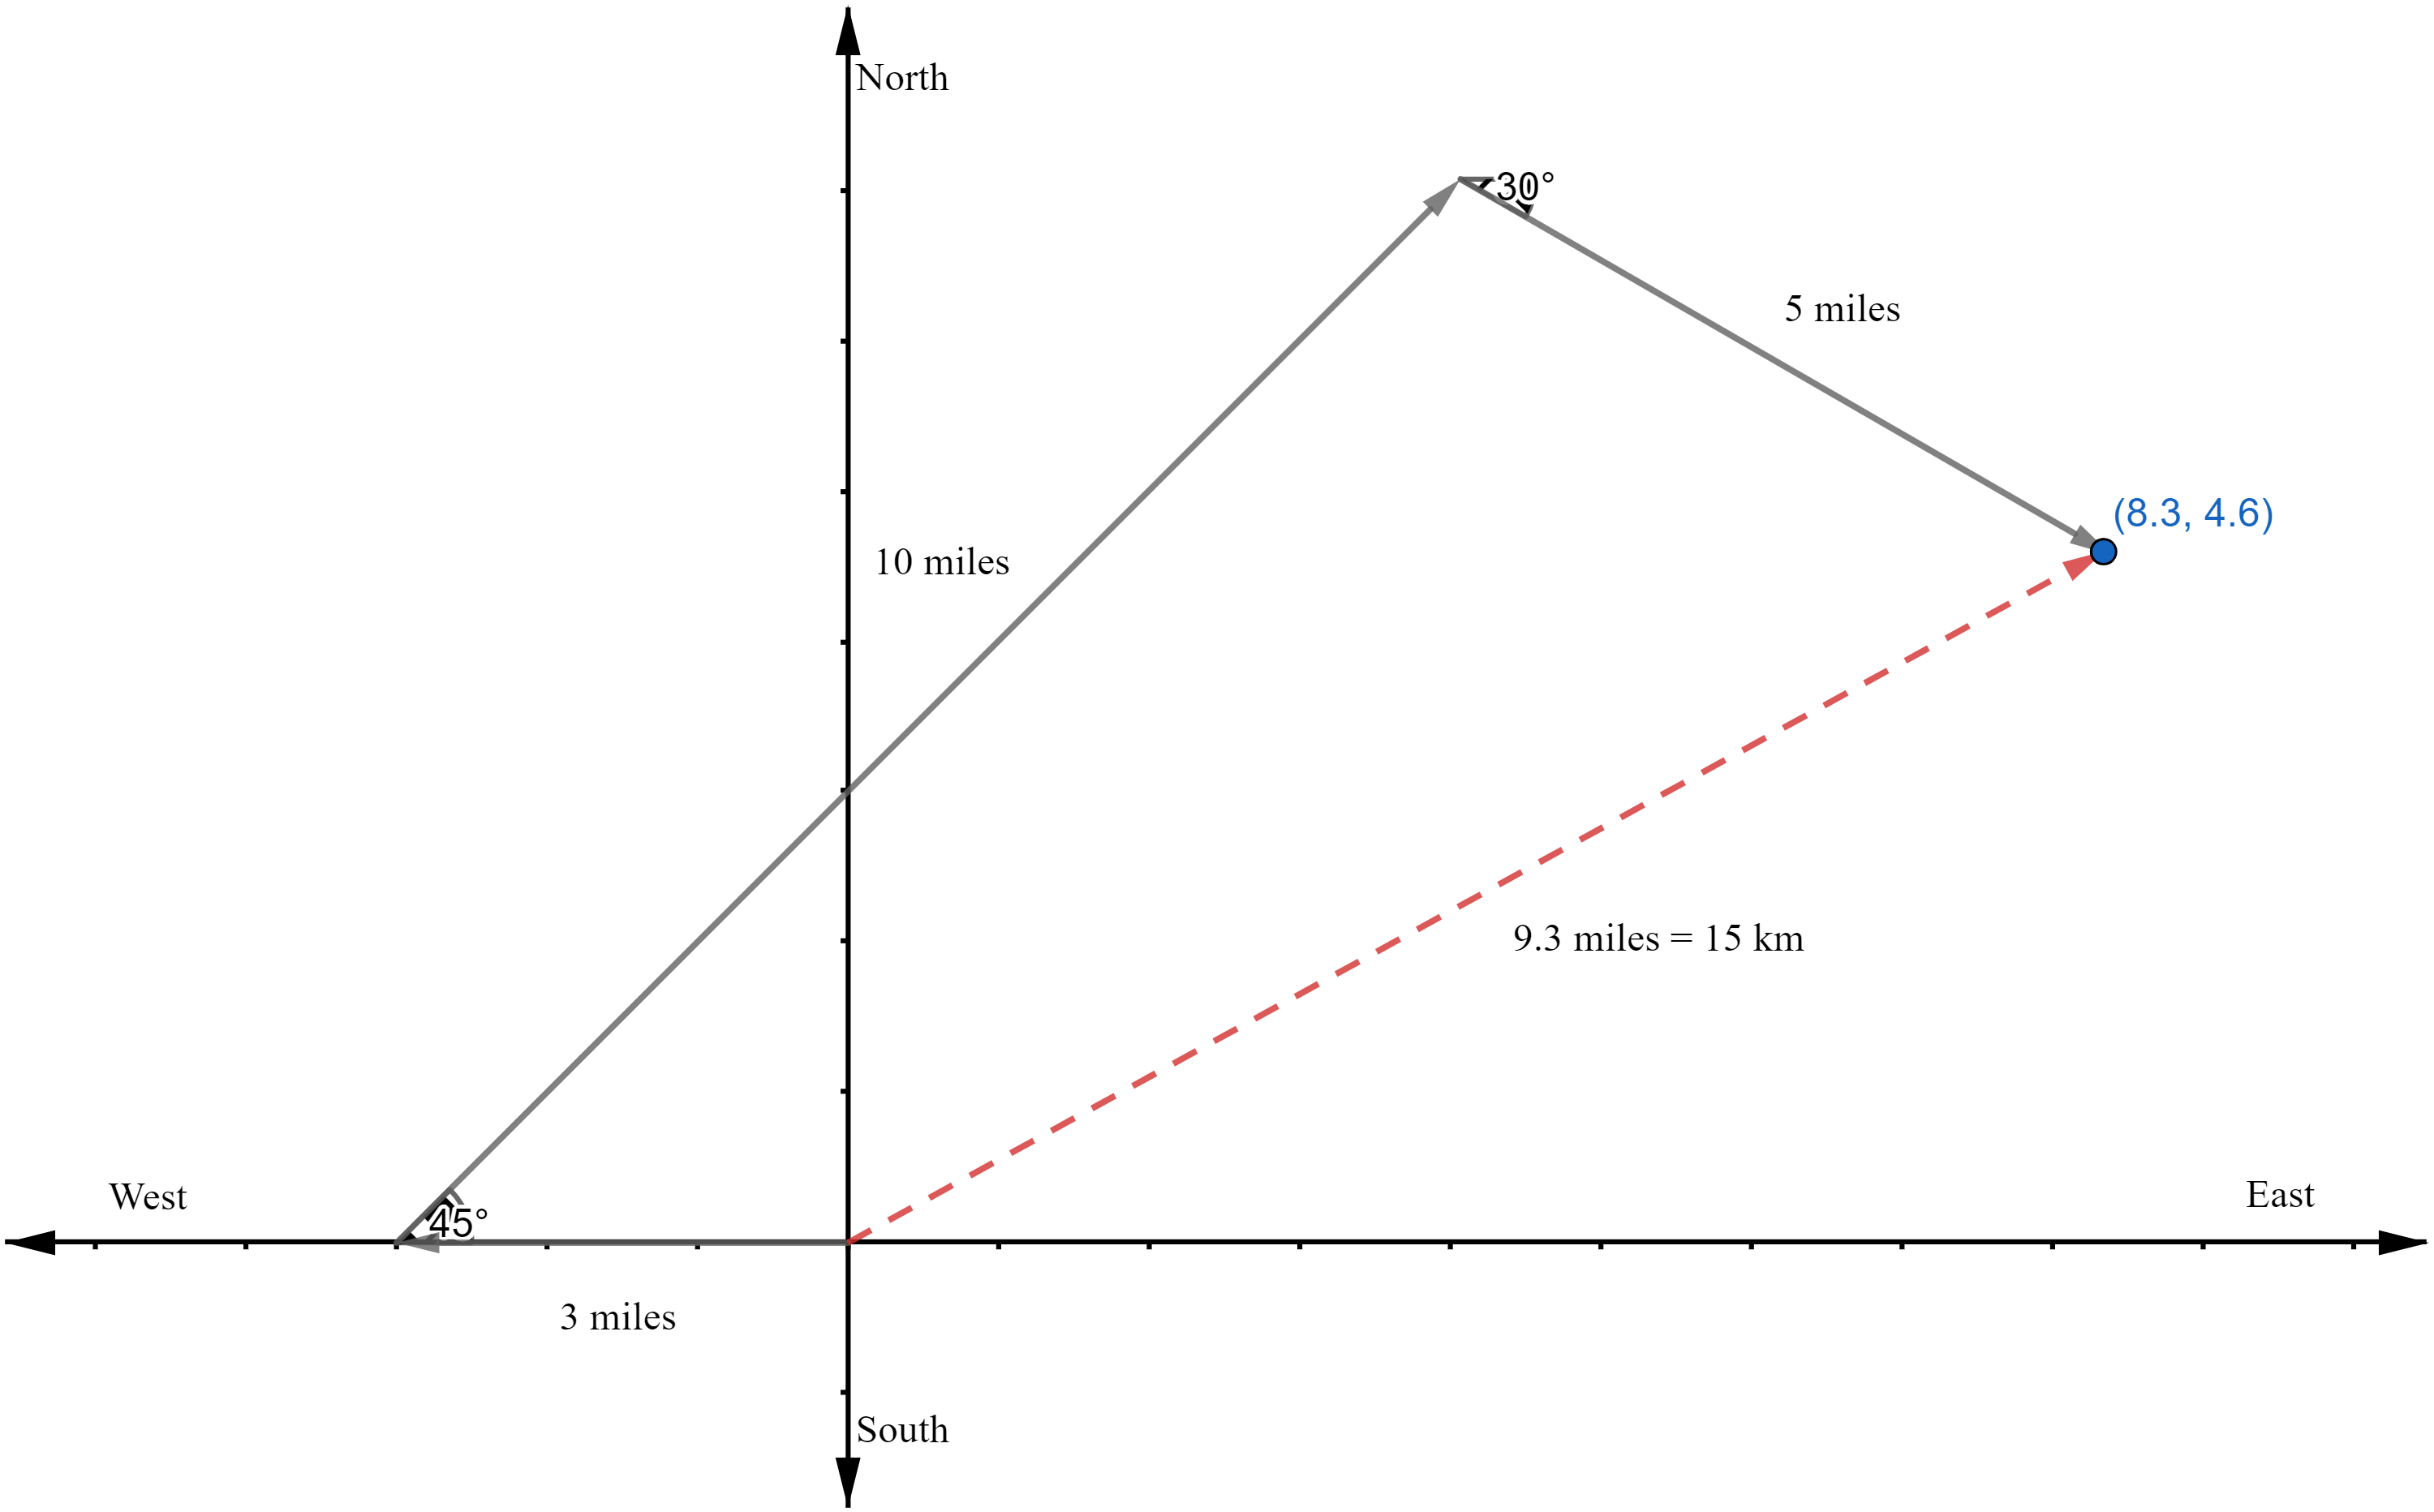
\includegraphics[width=\linewidth]{2.a.png}
    \end{center}
    \item
    Let the first vector be $\vec{V_{1}}$, the second $\vec{V_{2}}$, the third $\vec{V_{3}}$, and the resultant displacement $\vec{S}$.
    \begin{align}
        \vec{V_{1}} &= -3\hat{i} \\
        \vec{V_{2}} &= 10\cos(45^\circ)\hat{i}+10\sin(45^\circ)\hat{j} \\ \\
        & = \frac{10}{\sqrt{ 2 }}\hat{i}+\frac{10}{\sqrt{ 2 }}\hat{j} \\
        \vec{V_{3}} &= 5\cos(-30)\hat{i}+5\sin (-30)\hat{j} \\
        & = \frac{5\sqrt{ 3 }}{2}\hat{i}-\frac{5}{2}\hat{j} \\
        \vec{S} & = \vec{V_{1}} + \vec{V_{2}} + \vec{V_{3}}\\
        &= \left( -3+\frac{10}{\sqrt{ 2 }}+\frac{5\sqrt{ 3 }}{2} \right)\hat{i}+\left( \frac{10}{\sqrt{ 2 }}-\frac{5}{2} \right)\hat{j} \\
        |\vec{S}| &\approx 9.6 miles = 15.4 km
    \end{align}


\end{enumerate}

%%%%%%%%%%%%%%%%%%%%
\item
\begin{align*}
    \vec{r_{1}} &= 2\hat{i}-\hat{j}+\hat{k} \\
    \vec{r_{2}} &= \hat{i}+3\hat{j}-2\hat{k}\\
    \vec{r_{3}} &= -2\hat{i}+\hat{j}-3\hat{k}\\
    \vec{r_{4}} &= 3\hat{i}+2\hat{j}+5\hat{k}
\end{align*}
%%%%%%%%%%%%%%%%%%%%

\begin{align}
    \vec{r_{4}} &= a\vec{r_{1}} + b\vec{r_{2}} + c\vec{r_{3}}\\
    3\hat{i}+2\hat{j}+5\hat{k} &= a(2\hat{i}-\hat{j}+\hat{k}) + b(\hat{i}+3\hat{j}-2\hat{k}) + c(-2\hat{i}+\hat{j}-3\hat{k}) \\
    &= 2a\hat{i}-a\hat{j}+a\hat{k} + b\hat{i}+3b\hat{j}-2b\hat{k} + -2c\hat{i}+c\hat{j}-3c\hat{k} \\
    &= (2a+b-2c)\hat{i} + (-a+3b+c)\hat{j} + (a-2b-3c)\hat{k}
\end{align}

\begin{align}
    3&=2a+b-2c \\
    2&=-a+3b+c \\
    5&=a-2b-3c \\
\end{align}

\begin{align}
	\begin{bmatrix}
		a \\
		b \\
		c
	\end{bmatrix}
    &=
	\begin{bmatrix}
		2 & 1 & -2 \,\, \\
	-1 & 3 & 1 \\
	1 & -2 & -3
	\end{bmatrix}^{-1}
	\times
	\begin{bmatrix}
		3 \\
		2 \\
		5
	\end{bmatrix} \\
	\begin{bmatrix}
		a \\
		b \\
		c
	\end{bmatrix}
    &=
	\begin{bmatrix}
		\frac{1}{2} & -\frac{1}{2} & -\frac{1}{2} \\
	    \frac{1}{7} & \frac{2}{7} & 0 \\
	    \frac{1}{14} & -\frac{5}{14} & -\frac{1}{2}
	\end{bmatrix}
	\times
	\begin{bmatrix}
		3 \\
		2 \\
		5
	\end{bmatrix} \\
	\begin{bmatrix}
		a \\
		b \\
		c
	\end{bmatrix}
    &=
	\begin{bmatrix}
		-2 \\
		1 \\
		-3
	\end{bmatrix}
\end{align}

\item $\vec{A}=\cos\theta_{1}\hat{i}+\sin\theta_{1}\hat{j}$ and $\vec{B}=\cos\theta_{2}\hat{i}+\sin\theta_{2}\hat{j}$.

\begin{align}
    \vec{A}\cdot \vec{B} &= \cos\theta_{1}\cos\theta_{2} + \sin\theta_{1}\sin\theta_{2}\\
    |\vec{A}||\vec{B}|\cos\theta &= \\
    |\vec{A}|=|\vec{B}|=1\implies \cos\theta &= \\
    \cos(\theta_{1}-\theta_{2}) &= \\
    \therefore \cos(\theta_{1}\pm\theta_{2}) &=  \cos\theta_{1}\cos\theta_{2} \mp \sin\theta_{1}\sin\theta_{2}
\end{align}

\begin{align}
    \vec{A}\times \vec{B}&=(\vec{A}_{y}\vec{B}_{z}-\vec{A}_{z}\vec{B}_{y})\hat{i}-(\vec{A}_{x}B_{z}-\vec{A}_{z}B_{x})\hat{j}+(\vec{A}_{x}B_{y}-\vec{A}_{y}B_{x})\hat{k} \\
    &=(\sin\theta_{1}\cos\theta_{2}-\cos\theta_{1}\sin\theta_{2})\hat{k} \impliedby \vec{A}_{z}=\vec{B}_{z}=0 \\
    |\vec{A}| |\vec{B}|\sin\theta n&= \\
     \sin\theta\hat{k} &= \\
    \sin(\theta_{1}-\theta_{2})\hat{k} &= \\
    \therefore  \sin(\theta_{1}\pm\theta_{2}) &= \sin\theta_{1}\cos\theta_{2}\pm\cos\theta_{1}\sin\theta_{2}
\end{align}

\item $\vec{r}&=x(t)\hat{i}+y(t)\hat{j}$ where $x(t)&=2\alpha t-\sin(\alpha t)$ and $y(t)=1-\cos(\alpha t)$.

\begin{enumerate}
    \item 
    \begin{align}
        \vec{v}&=\vec{v}_{x}\hat{i}+\vec{v}_{y}\hat{j} \\
        &=\frac{d\vec{r}_{x}}{dt}\hat{i}+\frac{d\vec{r}_{y}}{dt}\hat{j} \\
        &=\frac{d[2\alpha t-\sin (\alpha t)]}{dt}\hat{i}+\frac{d[1-\cos(\alpha t)]}{dt}\hat{j} \\
        &= [2\alpha-\alpha \cos(\alpha t)]\hat{i}+\alpha \sin(\alpha t)\hat{j}
    \end{align}

    \item 
        \begin{align}
            \vec{v} &= \vec{v}_{r}+\vec{v}_{n} \\
            \vec{v}_{r}&=[2\alpha t-\sin(\alpha t)]\hat{i}+[1-\cos(\alpha t)]\hat{j} \\
            \vec{v}_{n}&=\frac{1}{2\alpha t-\sin(\alpha t)}\hat{i}-\frac{1}{1-\cos(\alpha t)}\hat{j} \\
        \end{align}
        \begin{align}
            \vec{v} &=
            \begin{bmatrix}
                2\alpha t-\sin(\alpha t) & 1-\cos(\alpha t) \\
                \dfrac{1}{2\alpha t-\sin(\alpha t)} & -\dfrac{1}{1-\cos(\alpha t)}
            \end{bmatrix}^{-1}
            \times
            \begin{bmatrix}
                2\alpha-\alpha \cos(\alpha t) \\
                \alpha \sin(\alpha t)
            \end{bmatrix} \\
                    &=
                    \begin{bmatrix}
                        \dfrac{-(-\sin(\alpha t)+2\alpha t)(2\alpha-\alpha \cos(\alpha t))-\alpha \sin\alpha t(-\sin(\alpha t)+2\alpha t)(1-\cos(\alpha t))^{2}}{-4\alpha^{2} t^{2}+4\alpha t\sin(\alpha t)-2} \\
                        \dfrac{-(1-\cos(\alpha t))(2\alpha-\alpha \cos(\alpha t))+\alpha \sin\alpha t(2\alpha t-\sin(\alpha t))^{2}(1-\cos(\alpha t))}{-4\alpha^{2} t^{2}+4\alpha t\sin(\alpha t)-2} \\
                    \end{bmatrix}
        \end{align}

\end{enumerate}

\end{enumerate}

\vfill

\begin{center}
    Made with \emoji{heart} in {\LaTeX}
\end{center}

\end{document}
